\documentclass{standalone}
\usepackage{tikz}
\usepackage{ctex,siunitx}
\setCJKmainfont{Noto Serif CJK SC}
\usepackage{tkz-euclide}
\usepackage{amsmath}
\usetikzlibrary{patterns, calc}
\usetikzlibrary {decorations.pathmorphing, decorations.pathreplacing, decorations.shapes,}
\begin{document}
\small
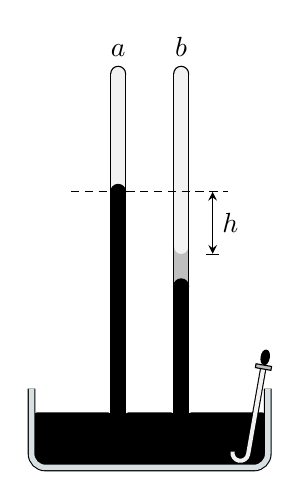
\begin{tikzpicture}[>=stealth,scale=1.0]
  \fill[rounded corners=5pt] (-1.5,0.5)rectangle(1.5,0);
  \fill[rounded corners=2pt] (-1.5,0.7)rectangle(-0.46,0.1);
  \fill[rounded corners=2pt] (-0.34,0.7)rectangle(0.34,0.1);
  \fill[rounded corners=2pt] (1.5,0.7)rectangle(0.46,0.1);
  \draw[double=cyan!20!gray!30,rounded corners=5pt,double distance=2pt] (-1.5,1)--(-1.5,0)--(1.5,0)--(1.5,1);
  \draw[double=black,double distance=5pt](0.4,0.5)--(0.4,2.3);
  \draw[double=black,double distance=5pt](-0.4,0.5)--(-0.4,3.5);
  \draw[fill=gray!10](-0.4,5.0)circle(2.7pt)node[above=1mm]{$a$}(0.4,5.0)circle(2.7pt)node[above=1mm]{$b$};
  \draw[double=gray!10,double distance=5pt](-0.4,3.5)--(-0.4,5);
  \draw[double=gray!50,double distance=5pt](0.4,2.8)--(0.4,2.3);
  \fill[gray!10](0.4,2.8)circle(2.5pt);
  \draw[double=gray!10,double distance=5pt](0.4,2.8)--(0.4,5.0);
  \draw[fill=black](-0.4,3.5)circle(2.7pt)(0.4,2.3)circle(2.7pt);
  \draw[thin,|<->](0.8,2.7)--(0.8,3.5)node[midway,right]{$h$};
  \draw[thin,densely dashed](-1,3.5)--(1,3.5);
  % \draw[double=gray!10,double distance=1.5pt](1.0,0.2)arc(170:350:0.1)--++(80:1.3);
  \coordinate (A) at (1.45,1.3);
  \coordinate (B) at ([shift=(80:0.2)]A);
  \fill(A)to[bend left=90](B)to[bend left=90](A);
  \draw[double=gray!10,double distance=1.5pt](A)--++(260:1.15)arc(350:170:0.1);
  \draw[fill=lightgray](A)--++(-10:0.1)--++(260:0.05)--++(170:0.2)--++(80:0.05)--cycle;
\end{tikzpicture}
\end{document}